\section{Literature Review}
\label{sec:Lit}
\par Give a \textbf{brief} overview of the theme, history and facts. You should use the present tense since what you are documenting is current knowledge. Do not dedicate a lot to historical facts about the subject matter, but limit to a paragraph. Make sure you quantify by quoting statistics where relevant. Following is an example for a research in \enquote{Automatic cyber-bullying detection}: \textit{With the popularity of social media, predominantly amongst the adolescent and young adult generations, there appears to be a correlation between the increase in suicide rates and social networking adoption~\cite{miron2019suicide}, with suicide attempts increasing by 10\% amongst adolescents and by 5.6\% amongst young adults for the period 2013-2017.} 

\par Due to shift towards “Industry 4.0”, companies were forced to seek automated solutions for hiring. With rise of Transformer-based models using Natural Language Inference (NLI), it allows machines to understand the intent behind a candidate’s story. Candidate's personality scoring relied on interviews, although unstrcuted interviews are known to be 20 to 30 percent predictable due to human error and human bias \cite{pansare2022pppkosam}. Since Natural Language processing has evolved, Large Language Models being the norm in every industry enables machines to score human personality traits from open ended response accurately. Literature review analyses use, performance, and accuracy of large language models in personality assesment 

\par A. Pansare, P. Panwar, and P. Kosamkar \cite{pansare2022pppkosam} conducted a comparative study on natural language processing systems based on predicting personalities. Researchers used an MBTI dataset containing 8670 rows (personality set and fifty recent tweets) and two columns where it represents mostly all personality types. All tweets collected and questionnaire was used to judge the participants personality. The system, developed by researchers, consists of Logistic Regression, Random Forest Algorithm, Support Vector Machines, and XGBoost. Results found that the system scored high accuracy scores with thinking/feeling attribute being the highest, but lowest being perceiving vs judging. 

\par S. R. Karra, S. T Nguyen, and T. Tulabandhula \cite{Karra:2022} conducted a comparative study from large language models on judging participants personality based on answers with use of Big Five Factors (Extraversion, Neuroticism, Agreeableness, Conscientiousness, Openness). Researchers used labels (each label has two ends such as from extroversion to introversion) on zero shot classifiers (ZSC), which are large language models, to judge the participants answers. Researchers used pre-processed datasets, from BookCorpus and Wikipedia, containing both sentences and small paragraphs for the ZSC to judge on. 

\par S. Sikström, I. Valavičiūtė, and P. Kajonius \cite{s2025sikstrom} analysed the validity of NLP judging personality based on word-based responses. 663 participants were recruited from United States of America, United Kingdom, and other countries with use of Prolific.io which is an online recruitment tool to collect data. The session consists of two phases. Phase 1 was where participants wrote a description about own or someone else’s specific personality trait with use of keywords and no mention of personality trait. Phase 2 was where other participants read participant’s written description. IPIP-NEO-30, derived from International Personality Item Pool, was used to measure, measured by participants, five personality factors, extraversion, openness, agreeableness, conscientiousness, and neuroticism. Demographic information such as age, gender, birth of country, education and confidence level were collected with use of questionnaires. The user-made descriptions, written in Microsoft Word, were analysed with use of GPT-4 and BERT based on the big five personality traits. Results found higher prediction accuracy than the rating scale, higher reliability, and better observation than self-report. 

\par J. Kurek et al. \cite{j2024kurek} conducted comparative study on zero shot classifier as a recruitment tool. Dataset contained unique job candidates, unique jobs, and matches between jobs and candidates totalling up to 3169 records. Only English documents were used only used due to researchers focus on English documents only. Models such as all-MiniLM-L2-v2 and LaBSe were selected by the researchers due to “models’ ability to produce embedding vector representations that accurately capture semantic meanings”. Results found high accuracy scores, importance of selecting the appropriate model as a recruitment tool, high performance, and recommended modifications on pre-trained models. 

\par L. Hu et al. \cite{lhu2024llm} made use of large language model (LLM) to analyse personality based on user’s input. Researchers collected user’s posts (from Kaggle and Pandora) which was used on LLM, GPT 3.5 Turbo, to analyse from three perspectives (semantic, sentiment, and linguistic perspective). Prompts were made to LLM to generate explanation on each MBTI trait and calculate similarity between the user and the label description with use of soft labels. Results found that the model, constructed by the researchers, outperformed all traditional methods that detect personalities, performance impact from focus on linguistic over semantic, and struggles to generate explanations with use of LLMs rather than specific small models. Limitations include limited dataset, and input length.

\par All sources touched on use of LLMs and NLPs in the context of job recruitment. Referenced studies made use of GPT-4, BERT, and BART as zero shot classifiers, and Logistic Regression, Random Forest, and XGBoost to predict personality traits from social media datasets. Pansare et al. \cite{pansare2022pppkosam} made use of specific models such as XGBoost, and Random Forest resulted in high accuracy but required large and pre-labelled datasets. On the other hand, Karra et al. \cite{Karra:2022} and Kurek et al. \cite{j2024kurek} employed Zero-shot classifiers showed that personality scoring was able to  be executed without specific training, supported by Sikstrom et al. \cite{s2025sikstrom} who found that GPT-4 offered high reliability than self-report scales. Although LLMs outperform traditional methods, LLMs often struggle to generate explanation based on traits compared to smaller specific models. In addition, Kurek et al. \cite{j2024kurek} identified a linguistic gap due to limiting found documents to only English, as well as Hu et al. finding performance gaps when focus shifts to linguistic perspectives over semantics. Limitations found in this literature review represent a knowledge gap that the research gap needed to be addressed in this research by using BART-MNLI to evaluate and score open-ended candidate stories. 

\par Finally, sources reviewed in the literature review were peer-reviewed and contained in-depth analysis, differed from non-academic sources that lacks evidential findings due to lack of analysis and use of biased sources. By putting focus on academic work, this literature review identified technical gaps such as linguistic constraints and bias driven by pretrained data. However, non-academic material would only provide benefits of use of AI, but do not provide any findings based on limitations found in academic work. 

\begin{table}[htbp]
\centering
\caption{Comparative Analysis of Literature: Data, Algorithms, and Metrics}
\label{tab:LitComparison}
\resizebox{\columnwidth}{!}{%
\begin{tabular}{|l|l|l|l|}
\hline
\textbf{Source} & \textbf{Data Set Type} & \textbf{Algorithm/Model} & \textbf{Primary Metric} \\ \hline
Pansare [1] & Social Media (MBTI) & XGBoost / Random Forest & Accuracy \\ \hline
Karra [2] & Wikipedia/Corpus & Zero-Shot (LLM) & Semantic Mapping \\ \hline
Sikström [3] & Prolific.io Narratives & GPT-4 / BERT & Pearson Correlation \\ \hline
Kurek [4] & Job-Matching Data & all-MiniLM / LaBSE & Matching Score \\ \hline
Hu [5] & Kaggle/Pandora Posts & GPT-3.5 Turbo & Soft Labels \\ \hline
\end{tabular}
}
\end{table}

\begin{figure}[ht]
    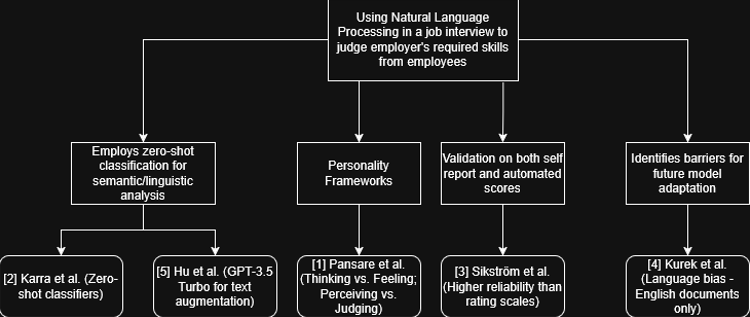
\includegraphics[scale=0.5]{includes/litmap.png}
    \centering
    \caption{Literature Map}
    \label{fig:Map}
\end{figure}